\documentclass[dvipdfmx,a4paper,13pt]{jsarticle}
\usepackage[deluxe]{otf}
\usepackage[top=20truemm,bottom=20truemm,left=15truemm,right=15truemm]{geometry}
\usepackage{multirow}
\usepackage{mhchem}
\usepackage{color}
\usepackage[dvipsnames]{xcolor}
\usepackage{enumerate}
\usepackage{tikz}
\usepackage{lscape}
\usepackage{amsmath}
\usepackage{chemfig}
\usepackage{fancyhdr}
\usepackage{lastpage}
\usepackage[dvipdfmx]{hyperref}
\usepackage{ascmac}
\usepackage{multicol}
\usepackage{amssymb}
\usetikzlibrary{calc}

\makeatletter
\def\section{\@startsection {section}{1}{\z@}{-2.5ex plus -1ex minus -.2ex}{2.5 ex plus .2ex}{\Large \bfseries \sffamily}}
\def\subsection{\@startsection {subsection}{1}{\z@}{-1.5ex plus -1ex minus -.2ex}{2.3 ex plus .2ex}{\Large \sffamily}}
\def\subsubsection{\@startsection {subsubsection}{1}{\z@}{-2.5ex plus -1ex minus -.2ex}{.3 ex plus .2ex}{\large \sffamily}}
\makeatother

\newcommand{\answer}[1]{\!
  \begin{tikzpicture}[baseline=(num.base),font=\sffamily\small]
   \node[draw=black, rectangle, rounded corners=2pt,
          text=black,
          line width=.5pt, inner sep=2pt, outer sep=0pt
          ] (num){\addtocounter{answer}{1}\arabic{answer}};
   \node [right, inner sep=1pt, outer sep=0pt] (text) at (num.east){#1};
   \draw [line width=.5pt, outer sep=0pt] (num.south)--($(text.base east)-(num.base west)+(num.south)+(-10pt,0)$);
  \end{tikzpicture}%
}
\newcounter{answer}
\newcommand{\hl}[1]{\answer{\textcolor{red}{#1}}}\newcommand{\hce}[1]{\textcolor{blue}{\ce{#1}}}\newcommand{\hlbox}[1]{\fbox{\textcolor{red}{\gtfamily #1}}}\rfoot{解答編}
%\newcommand{\hl}[1]{\answer{\phantom{あいう}}}\newcommand{\hce}[1]{\fbox{\textcolor{white}{\ce{#1}}}}\newcommand{\hlbox}[1]{\fbox{\phantom{#1}}}\rfoot{空欄編}

\pagestyle{empty}

\newcommand{\stamp}[2]{%
  \begin{tikzpicture}[baseline=(A.base),font=\sffamily\small]
    \node[draw=#1, rectangle, rounded corners=2pt,
          text=#1,
          fill=#1!10!white,
          line width=.4pt, inner sep=1pt, outer sep=0pt
          ] (A) {#2};
  \end{tikzpicture}%
}
\newcommand{\K}{\stamp{blue}{工業的製法}}
\newcommand{\R}{\stamp{red}{例}}

\columnseprule=0.2mm

\pagestyle{fancy}
\lfoot{\hyperlink{top}{無機化学}}
\cfoot{\thepage/\pageref{LastPage}}

\hypersetup{
 bookmarks=false,
 colorlinks=true,
 linkcolor=black,
 citecolor=[rgb]{0,0.4,0.8},
 filecolor=black,
 urlcolor=[rgb]{0,0.4,0.8}
}

\begin{document}

%\setchemfig{debug=true}
%\setcharge{debug}

\thispagestyle{fancy}

\twocolumn
\twocolumn[
\begin{center}
\Huge{\gtfamily 無機化学}\\
\vspace{5mm}
\end{center}
]
\hypertarget{top}{\tableofcontents}
\twocolumn[
\newpage
 \part{非金属元素}
 ]
 \section{水素}
  \subsection{性質}
  \begin{itemize}
   \item \hl{無}色\hl{無}臭の\hl{気体}
   \item 最も\hl{軽い}
   \item 水に溶け\hl{にくい}
  \end{itemize}
  \subsection{同位体}
  \ce{_{}^{1}H} 99\%以上 \ce{_{}^{2}H} (\hl{D})0.015\% \ce{_{}^{3}H} (\hl{T})微量
  \subsection{製法}
  \begin{itemize}
   \item ナフサの電気分解 \K
  \item \hl{赤熱したコークス}に\hl{水蒸気}を吹き付ける \K\\
  \hce{C + H2O -> H2 + CO}
  \item \hl{水}(\hl{水酸化ナトリウム水溶液})の電気分解\\
  \hce{2H2O -> 2H2 + O2}
  \item \hl{イオン化傾向}が\hl{\ce{H2}より大きい}金属と希薄強酸\\
  \R \;\ce{Fe + 2HCl -> FeCl2 + H2 ^}\\
  \R \;\ce{Zn + 2HCl -> ZnCl2 + H2 ^}
  \item 水素化ナトリウムと水\\
  \hce{NaH + H2O -> NaOH + H2}
 \end{itemize}
 \subsection{反応}
 \begin{itemize}
  \item 水素と酸素(爆鳴気の燃焼)\\
  \hce{2H2 + O2 -> H2O}
  \item 加熱した酸化銅(\ajRoman{2})と水素\\
  \hce{CuO + H2 -> Cu + H2O}
 \end{itemize}
 \newpage
 \section{貴ガス}
 \hl{\ce{He}}, \hl{\ce{Ne}}, \hl{\ce{Ar}}, \hl{\ce{Kr}}, \ce{Xe}, \ce{Rn}
  \subsection{性質}
  \begin{itemize}
   \item \hl{無}色\hl{無}臭
   \item 第18族元素であり、電子配置がオクテットを満たすため反応性が低い
   \item イオン化エネルギーが極めて大きい
   \item 電子親和力が\hl{極めて小さい}
   \item 電気陰性度が\hl{定義されない}
  \end{itemize}
  \subsection{生成}
  \ce{_{}^{40}K}の電子捕獲\\
  \quad\hce{_{}^{40}K + e- -> _{}^{40}Ar}
  \subsection{ヘリウム}
  化学式:\ce{He}
  浮揚ガス
  \subsection{ネオン}
  化学式:\ce{Ne}
  ネオンサイン
  \subsection{アルゴン}
  化学式:\ce{Ar}
  \ce{N2}, \ce{O2}に次いで3番目に空気中での存在量が多い(約1\%)。
  
 \newpage
 \onecolumn
 \section{ハロゲン}
  \subsection{単体}
  \subsubsection{性質}
  \begin{center}
  \begin{tabular}{|c||c|c|c|c|}\hline
   化学式&\ce{F2}&\ce{Cl2}&\ce{Br2}&\ce{I2}\\ \hline\hline
   分子量&\multicolumn{4}{|c|}{小 \quad\tikz \draw[line width=0.5pt] (10,0.1)--(0,0)--(10,-0.1);\quad 大}\\ \hline
   分子間力&\multicolumn{4}{|c|}{弱 \quad\tikz \draw[line width=0.5pt] (10,0.1)--(0,0)--(10,-0.1);\quad 強}\\ \hline
   反応性&\multicolumn{4}{|c|}{強 \quad\tikz \draw[line width=0.5pt] (0,0.1)--(10,0)--(0,-0.1);\quad 弱}\\ \hline
   沸点・融点&\multicolumn{4}{|c|}{低 \quad\tikz \draw[line width=0.5pt] (10,0.1)--(0,0)--(10,-0.1);\quad 高}\\ \hline
   常温での状態&\hl{気体}&\hl{気体}&\hl{液体}&\hl{固体}\\ \hline
   色&\hl{淡黄}色&\hl{黄緑}色&\hl{赤褐}色&\hl{黒紫}色\\ \hline
   特徴&\hl{特異}臭&\hl{刺激}臭&揮発性&\hl{昇華}性\\ \hline
   \ce{H2}との反応&
   \begin{tabular}{c}
   \hl{冷暗所}でも\\爆発的に反応
   \end{tabular}&
   \begin{tabular}{c}
   \hl{常温}でも\hl{光}で\\爆発的に反応
   \end{tabular}&
   \begin{tabular}{c}
   \hl{加熱}して\\\hl{触媒}により反応
   \end{tabular}&
   \begin{tabular}{c}
   高温で平衡状態\\
   \hl{加熱}して\hl{触媒}により一部反応
   \end{tabular}\\ \hline
   水との反応&
   \begin{tabular}{c}
   水を酸化して酸素と\\
   \hl{激しく}反応
   \end{tabular}&
   \hl{一部とけて反応}&
   \hl{一部とけて反応}&
   \begin{tabular}{c}
   \hl{反応しない}\\\hl{\ce{KIaq}には可溶}
   \end{tabular}\\ \hline
   用途&
   \begin{tabular}{c}
   保存が困難\\
   \ce{Kr}や\ce{Xe}と反応
   \end{tabular}&
   \begin{tabular}{c}
   \hl{\ce{ClO-}}による\\\hl{殺菌・漂白}作用
   \end{tabular}&
   \begin{tabular}{c}
   \ce{C=C}や\\
   \ce{C#C}の検出
   \end{tabular}&
   \begin{tabular}{c}
   \hl{ヨウ素デンプン}反応で\\
   \hl{青紫}色
   \end{tabular}\\ \hline
  \end{tabular}
  \end{center}
\begin{multicols}{2}
  \subsubsection{製法}
   \begin{itemize}
    \item フッ化水素ナトリウム\ce{KHF2}のフッ化水素\ce{HF}溶液の電気分解 \K\\
    \ce{KHF2 -> KF + HF}
    \item \hl{塩化ナトリウム水溶液}の電気分解 \stamp{teal}{塩素} \K\\
    \hce{2NaCl + 2H2O -> Cl2 + H2 + 2NaOH}
    \item \hl{酸化マンガン(\ajRoman{4})}に\hl{濃塩酸}を加えて加熱 \stamp{teal}{塩素}\\
    \hce{MnO2 + 4HCl ->[][\Delta] MnCl2 + Cl2 ^ + 2H2O}
    \item \hl{高度さらし粉}と\hl{塩酸} \stamp{teal}{塩素}\\
    \hce{Ca(ClO)2*2H2O + 4HCl -> CaCl2 + 2Cl2 ^ + 4H2O}
    \item \hl{さらし粉}と\hl{塩酸} \stamp{teal}{塩素}\\
    \hce{CaCl(ClO)*H2O + 2HCl -> CaCl2 + Cl2 ^ + 2H2O}
    \item 臭化マグネシウムと塩素 \stamp{teal}{臭素}\\
    \ce{MgBr2 + Cl2 -> MgCl2 + Br2}
    \item ヨウ化カリウムと塩素 \stamp{teal}{ヨウ素}\\
    \ce{2KI + Cl2 -> 2KCl + I2}
   \end{itemize}
  \columnbreak
  \subsubsection{反応}
  \begin{itemize}
   \item フッ素と水素\\
   \hce{H2 + F2 ->T[常温で爆発的に反応] 2HF}
   \item 塩素と水素\\
   \hce{H2 + Cl2 ->T[光を当てると爆発的に反応] 2HCl}
   \item 臭素と水素\\
   \hce{H2 + Br2 ->T[高温で反応] 2HBr}
   \item ヨウ素と水素\\
   \hce{H2 + I2 <=>T[高温で平衡] 2HI}
   \item フッ素と水\\
   \hce{2F2 + 2H2O -> 4HF + O2}
   \item 塩素と水\\
   \hce{Cl2 + H2O <=> HCl + HClO}
   \item 臭素と水\\
   \hce{Br2 + H2O <=> HBr + HBrO}
   \item ヨウ素の固体がヨウ化物イオン存在下で三ヨウ化物イオンを形成して溶解する反応\\
   \hce{I2 + I- -> I3-}
  \end{itemize}
\end{multicols}
\newpage
  \subsubsection{塩素発生実験の装置}
  \ce{MnO2 + 4HCl ->[][\Delta] MnCl2 + Cl2 ^ + 2H2O}\\
  \ce{Cl2},\ce{HCl},\ce{H2O}\\
  ↓\hl{\quad 水\quad}に通す (\ce{HCl}の除去)\\
  \ce{Cl2},\ce{H2O}\\
  ↓\hl{濃硫酸}に通す (\ce{H2O}の除去)\\
  \ce{Cl2}
  \subsubsection{塩素のオキソ酸}
  オキソ酸$\cdots$\hl{酸素を含む酸性物質}\\\\
   \begin{tabular}{r|lrl}
    +\ajRoman{7}&\hl{\ce{HClO4}}&\hl{\quad 過塩素酸}&\hlbox{\chemfig{H-[,0.6]O-[,0.6]Cl(-[:90,0.6]O)(-[:-90,0.6]O)-[,0.6]O}}\\\hline
    +\ajRoman{5}&\hl{\ce{HClO3}}&\hl{\qquad 塩素酸}&\hlbox{\chemfig{H-[,0.6]O-[,0.6]Cl(-[:90,0.6]O)-[,0.6]O}}\\\hline
    +\ajRoman{3}&\hl{\ce{HClO2}}&\hl{\quad 亜塩素酸}&\hlbox{\chemfig{H-[,0.6]O-[,0.6]Cl-[,0.6]O}}\\\hline
    +\ajRoman{1}&\hl{\ce{HClO}}&\hl{次亜塩素酸}&\hlbox{\chemfig{H-[,0.6]O-[,0.6]Cl}}\\
   \end{tabular}
  \subsection{ハロゲン化水素}
   \subsubsection{性質}
   \begin{table}[hbtp]
   \begin{tabular}{|c||c|c|c|c|}\hline
   化学式&\ce{HF}&\ce{HCl}&\ce{HBr}&\ce{HI}\\ \hline
   色・臭い&\multicolumn{4}{|c|}{\hl{無}色\hl{刺激}臭}\\ \hline
   沸点&$20^\circ$C&$-85^\circ$C&$-67^\circ$C&$-35^\circ$C\\ \hline
   水との反応&\multicolumn{4}{|c|}{\hl{よく溶ける}}\\ \hline
   水溶液&\multicolumn{1}{c}{\hl{フッ化水素酸}}&\multicolumn{1}{c}{\hl{塩酸}}&\multicolumn{1}{c}{\hl{臭化水素酸}}&\hl{ヨウ化水素酸}\\
   (強弱)&
   \multicolumn{4}{|c|}{
   \begin{tabular}{ccccccc}
   \hl{弱酸}&$\ll$&\hl{強酸}&$<$&\hl{強酸}&$<$&\hl{強酸}
   \end{tabular}
   }\\ \hline
   用途&
   \begin{tabular}{c}
   \hl{ガラス}と反応\\
   $\Rightarrow$ ポリエチレン瓶
   \end{tabular}&
   \begin{tabular}{c}
   \hl{アンモニア}の検出\\
   各種工業
   \end{tabular}&
   半導体加工&
   \begin{tabular}{c}
   インジウムスズ\\
   酸化物の加工
   \end{tabular}
   \\ \hline
   \end{tabular}
   \end{table}
   \subsubsection{製法}
    \begin{itemize}
     \item \hl{ホタル石}に\hl{濃硫酸}を加えて加熱(\hl{弱酸遊離}) \stamp{teal}{フッ化水素}\\
     \hce{CaF2 + H2SO4 ->[][\Delta] CaSO4 + 2HF ^}
     \item \hl{水素}と\hl{塩素} \stamp{teal}{塩化水素} \K\\
     \hce{H2 + Cl2 -> 2HCl ^}
     \item \hl{塩化ナトリウム}に\hl{濃硫酸}を加えて加熱  \stamp{teal}{塩化水素}(\hl{弱}酸・\hl{揮発性}酸の追い出し)\\
     \hce{NaCl + H2SO4 ->[][\Delta] NaHSO4 + HCl ^}
    \end{itemize}
   \subsubsection{反応}
   \begin{itemize}
    \item 気体のフッ化水素がガラスを侵食する反応\\
    \hce{SiO2 + 4HF(g) -> SiF4 ^ + 2H2O}
    \item フッ化水素酸(水溶液)がガラスを侵食する反応\\
    \hce{SiO2 + 6HF(aq) -> H2SiF6 ^ + 2H2O}
    \item \hl{塩化水素}による\hl{アンモニア}の検出\\
    \hce{HCl + NH3 -> NH4Cl}
   \end{itemize}
  \subsection{ハロゲン化銀}
  \subsubsection{性質}
  \begin{tabular}{|c||c|c|c|c|}\hline
  化学式&\ce{AgF}&\ce{AgCl}&\ce{AgBr}&\ce{AgI}\\ \hline
  固体の色&\hl{黄褐}色&\hl{白}色&\hl{淡黄}色&\hl{黄}色\\ \hline
  水との反応&\hl{よく溶ける}&\multicolumn{3}{|c|}{\hl{ほとんど溶けない}}\\ \hline
  光との反応&\hl{感光}&\multicolumn{3}{|c|}{感光性(→\hl{\ce{Ag}})}\\ \hline
  \end{tabular}\\
  \subsubsection{製法}
  \begin{itemize}
   \item 酸化銀(\ajRoman{1})にフッ化水素酸を加えて蒸発圧縮\\
   \hce{Ag2O + 2HF -> 2AgF + H2O}
   \item ハロゲン化水素イオンを含む水溶液と\hl{硝酸銀水溶液}\\
   \hce{Ag+ + X- -> AgX v}
  \end{itemize}
  \subsection{次亜塩素酸塩}
  \subsubsection{性質}
  \hl{酸化}剤として反応(\hl{殺菌}・\hl{漂白}作用)\\
  \quad \hce{ClO- + 2H+ + 2e- -> Cl- + H2O}
  \subsubsection{製法}
  \begin{itemize}
   \item 水酸化ナトリウム水溶液と塩素\\
   \hce{2NaOH + Cl2 -> NaCl + NaClO + H2O}
   \item 水酸化カルシウムと塩素\\
   \hce{Ca(OH)2 + Cl2 -> CaCl(ClO)*H2O}
  \end{itemize}
  \subsection{塩素酸カリウム}
  化学式:\hl{\ce{KClO3}}
  \subsubsection{性質}
  \hl{酸素}の生成(\hl{二酸化マンガン}を触媒に加熱)\\
  \quad \hce{2KClO3 ->C[MnO2][\Delta] 2KCl + 3O2 ^}
  
 \newpage
 \section{酸素}
  \subsection{酸素原子}
  同\hl{位}体:酸素(\ce{O2}),\hl{オゾン}(\ce{O3})\\
  \quad 地球の地殻に\hl{最も多く}存在
   \begin{itembox}[l]{地球の地殻における元素の存在率}
   \begin{tabular}{ccccccccccc}
   \hl{\ce{O}} & \multirow{2}{*}{$>$} & \hl{\ce{Si}} & \multirow{2}{*}{$>$} & \hl{\ce{Al}} & \multirow{2}{*}{$>$} & \hl{\ce{Fe}} & \multirow{2}{*}{$>$} & \hl{\ce{Ca}} & \multirow{2}{*}{$>$} & \hl{\ce{Na}}\\
   \hl{酸素}&&\hl{ケイ素}&&\hl{アルミニウム}&&\hl{鉄}&&\hl{カルシウム}&&\hl{ナトリウム}\\
   46.6\%&&27.7\%&&8.13\%&&5.00\%&&3.63\%&&2.83\% \\
   おっ&&し&&ゃる&&て&&か&&な
   \end{tabular}
   \end{itembox}
   
 \begin{multicols}{2}
  \subsection{酸素}
   化学式:\ce{O2}
   \subsubsection{性質}
   \begin{itemize}
   \item \hl{無}色\hl{無}臭の\hl{気体}
   \item 沸点 $-183^\circ$C
   \end{itemize}
   \subsubsection{製法}
   \begin{itemize}
    \item \hl{液体空気の分留} \K
    \item \hl{水}(\hl{水酸化ナトリウム水溶液})の\hl{電気分解}\\
    \hce{2H2O -> 2H2 ^ + O2 ^}
    \item \hl{過酸化水素水}(\hl{オキシドール})の分解\\
    \hce{2H2O2 ->C[MnO2] O2 ^ + 2H2O}
    \item \hl{塩素酸カリウム}の熱分解\\
    \hce{2KClO3 ->C[MnO2][\Delta] 2KCl + 3O2 ^}
   \end{itemize}
   \subsubsection{反応}
   
   \hl{酸化}剤としての反応\\
   \quad \hce{O2 + 4H+ + 4e- -> 2H2O}
  \subsection{オゾン}
   化学式:\hl{\ce{O3}}
   \subsubsection{性質}
   \begin{itemize}
    \item \hl{ニンニク}臭(\hl{特異}臭)を持つ\hl{淡青}色の\hl{気体}(常温)
    \item 水に\hl{少し溶ける}
    \item \hl{殺菌}・\hl{脱臭}作用
   \end{itemize}
   \columnbreak
   \begin{itembox}[l]{オゾンにおける酸素原子の運動}
   \begin{center}
   \chemfig{\charge{[circle]30=\.,150=\:,270=\:}{O}-[:30,0.6,,,opacity = 0]\charge{[circle]90=\:,210=\.,330=\:}{O}=[:-30,0.6,,,opacity = 0]\charge{[circle]30=\:,150=\:,270=\:}{O}}
   \ce{<=>T[\hl{共鳴}]} 
   \chemfig{\charge{[circle]30=\:,150=\:,270=\:}{O}-[:30,0.6,,,opacity = 0]\charge{[circle]90=\:,210=\:,330=\.}{O}=[:-30,0.6,,,opacity = 0]\charge{[circle]30=\:,150=\.,270=\:}{O}}
   \end{center}
   \hfill $\Rightarrow$\hl{極性}
   \end{itembox}
   \subsubsection{製法}
   酸素中で\hl{無声放電}/強い\hl{紫外線}を当てる\\
   \quad \hce{3O2 -> 2O3}
   \subsubsection{反応}
   \begin{itemize}
   \item \hl{酸化}剤としての反応\\
   \hce{O3 + 2H+ + 2e- -> O2 + H2O}
   \item 湿らせた\hl{ヨウ化カリウムでんぷん紙}を\hl{青}色に変色\\
   \hce{O3 + 2KI + H2O -> I2 + O2 + 2KOH}
   \end{itemize}
 \end{multicols}
  \subsection{酸化物}
  \begin{tabular}{|c|c|c|c|}\hline
  &塩基性酸化物&両性酸化物&酸性酸化物\\ \hline
  元素&\hl{陽性の大きい金属}元素&\hl{陽性の小さい金属}元素&\hl{非金属}元素\\ \hline
  水との反応&\hl{塩基性}&\hl{ほとんど溶けない}&\hl{酸性}(\hl{オキソ酸})\\ \hline
  中和&\hl{酸}と反応&\hl{酸・塩基}と反応&\hl{塩基}と反応\\ \hline
  \end{tabular}\\
  両性酸化物$\cdots$\hl{アルミニウム}(\hl{Al}),\hl{亜鉛}(\hl{Zn}),\hl{スズ}(\hl{Sn}),\hl{鉛}(\hl{Pb})\footnote{覚え方:ああすんなり}
  \begin{enumerate}[\R]
   \item \ce{CO2 + H2O -> H2CO3}
   \item \ce{SO2 + H2O -> H2SO3}
   \item \ce{3NO2 + H2O -> 2HNO3 + NO}
  \end{enumerate}
  \subsubsection{反応}
  \begin{itemize}
   \item 酸化銅(\ajRoman{2})と塩化水素\\
   \hce{CuO + 2HCl -> CuCl2 + H2O}
   \item 酸化アルミニウムと硫酸\\
   \hce{Al2O3 + 3H2SO4 -> Al2(SO4)3 + 3H2O}
   \item 酸化アルミニウムと水酸化ナトリウム水溶液\\
   \hce{Al2O3 + 2NaOH + 3H2O -> 2Na[Al(OH)4]}
  \end{itemize}
  \subsection{水}
  \subsubsection{性質}
  \begin{multicols}{2}
  \begin{itemize}
   \item \hl{極性}分子
   \item 周りの4つの分子と\hl{水素}結合
   \item 異常に\hl{高い}沸点
   \item \hl{隙間の多い}結晶構造(密度:固体\hl{<}液体)
   \item 特異な\hl{融解曲線}
  \end{itemize}
  \subsubsection{反応}
  \begin{itemize}
   \item 酸化カルシウムと水\\
   \hce{CaO + H2O -> Ca(OH)2}
   \item 二酸化窒素と水\\
   \hce{3NO2 + H2O -> 2HNO3 + NO}
  \end{itemize}

  \columnbreak
  \chemfig{H(-[:190,0.7,,,black,line width=2pt,dash pattern=on 1pt off 2pt]O(-[::-40,0.7]H)-[::40,0.7]H)-[:10]O(-[:90,0.9,,,black,line width=2pt,dash pattern=on 1pt off 2pt]H-[:120,0.7]O-[:200,0.7]H)(-[:-10,,,,black,line width=2pt,dash pattern=on 1pt off 2pt]H-[:40,0.7]O-[:-40,0.7]H)-[:-60,0.9]H-[:-60,0.7,,,black,line width=2pt,dash pattern=on 1pt off 2pt]O(-[,0.7]H)-[:-80,0.7]H}
  \end{multicols}
 \section{硫黄}
  \subsection{硫黄}
   \subsubsection{性質}
   \begin{tabular}{|c||c|c|c|}\hline
   名称&\hl{斜方}硫黄&\hl{単斜}硫黄&\hl{ゴム状}硫黄\\ \hline
   化学式&\hl{\ce{S8}}&\hl{\ce{S8}}&\hl{\ce{S_{$x$}}}\\ \hline \hline
   色&\hl{黄}色&\hl{黄}色&\hl{黄}色\\ \hline
   構造&\hl{塊状}結晶&\hl{針状}結晶&\hl{不定形}固体\\ \hline
   融点&$113^\circ$C&$119^\circ$C&不定\\ \hline
   構造&\multicolumn{2}{|c|}{\chemfig{S?-[:-30,0.57735]S-[:30,0.57735]S-[:-30,0.57735]S-[:30,0.57735]S-[:-120]S-[:135,0.7071]S-[:-135,0.7071]S?}}&\chemfig{-[:30,0.5,,,black,line width=2pt,dash pattern=on 1pt off 2pt]S-[:30,0.7]S-[::-90,0.7]S-[::100,0.7]S-[::-100,0.7]S-[::-60,0.7]S-[::-60,0.7]S-[::0,0.5,,,black,line width=2pt,dash pattern=on 1pt off 2pt]}\\ \hline
   \ce{CS2}との反応&\hl{溶ける}&\hl{溶ける}&\hl{溶けない}\\ \hline
   \end{tabular}\\
   \ce{CS2}$\cdots$無色・芳香性・揮発性$\Rightarrow$\hl{無極性}触媒
   \subsubsection{反応}
   \begin{itemize}
    \item 高温で多くの金属(\ce{Au}, \ce{Pt}を除く)と反応\\
    \R \ce{Fe} \hce{Fe + S -> FeS}
    \item 空気中で\hl{青}色の炎を上げて燃焼\\
    \hce{S + O2 -> SO2}
   \end{itemize}
  \subsection{硫化水素}
   化学式:\hl{\ce{H2S}}
   \subsubsection{性質}
   \begin{itemize}
    \item \hl{無}色\hl{腐卵}臭
    \item \hl{弱酸}性\\$\left\{
    \begin{tabular}[h]{ll}
    \hl{\ce{H2S <=> H+ + HS-}}& $K_{1}=9.5\times10^{-8}$ mol/L\\
    \hl{\ce{HS- <=> H+ + S^2-}}& $K_{2}=1.3\times10^{-14}$ mol/L
    \end{tabular}
    \right.$
    \item \hl{還元}剤としての反応\\
    \hce{H2S -> S + 2H+ + 2e-}
    \item 重金属イオン\ce{M^2+}と\hl{難容性の塩}を生成\\
    \hce{M2+ + S^{2-} <=> MS v}
   \end{itemize}
   \subsubsection{製法}
   \begin{itemize}
    \item 硫化鉄(\ajRoman{2})と希塩酸\\
    \hce{FeS + 2HCl -> FeCl2 + H2S ^}
    \item 硫化鉄(\ajRoman{2})と希硫酸\\
    \hce{FeS + H2SO4 -> FeSO4 + H2S ^}
   \end{itemize}
   \subsubsection{反応}
   \begin{itemize}
    \item 硫化水素とヨウ素\\
    \hce{H2S + I2 -> S + 2HI}
    \item 酢酸鉛(\ajRoman{2})水溶液と硫化水素(\hl{\ce{H2S}}の検出)\\
    \hce{(CH3COO)2Pb + H2S -> 2CH3COOH + PbS v}
   \end{itemize}
  \subsection{二酸化硫黄(亜硫酸ガス)}
  化学式:\hl{\ce{SO2}}
  電子式:\quad\hlbox{\chemfig{\charge{[circle]0=\:,90=\:,180=\:,270=\:}{O}-[-2,0.5,,,opacity=0]\charge{[circle]0=\:,-90=\:}{S}-[,0.6,,,opacity=0]\charge{[circle]90=\:,180=\:,270=\:}{O}}}
  \subsubsection{性質}
  \begin{itemize}
   \item \hl{無}色、\hl{刺激}臭の\hl{気体}
   \item 水に\hl{溶けやすい}
   \item \hl{弱酸}性\\
    \begin{tabular}{ll}
    \hl{\ce{SO2 + H2O <=> H+ + HSO3-}}& $K_{1}=1.4\times10^{-2}$ mol/L\\
    \end{tabular}
   \item \hl{還元}剤(\hl{漂白}作用)\\
   \hce{SO2 + 2H2O -> SO4^2- + 4H+ + 2e-}
   \item \hl{酸化}剤(\hl{\ce{H2S}}などの強い還元剤に対して)\\
   \hce{SO2 + 4H+ + 4e- -> S + 2H2O}
  \end{itemize}
  \subsubsection{製法}
  \begin{itemize}
   \item 硫黄や硫化物の\hl{燃焼} \K\\
   \hce{2H2S + 3O2 -> 2SO2 + 2H2O}
   \item \hl{亜硫酸ナトリウム}と{希硫酸}\\
   \hce{Na2SO3 + H2SO4 ->[][\Delta] Na2SO4 + SO2 ^ + H2O}
   \item \hl{銅}と\hl{熱濃硫酸}\\
   \hce{Cu + 2H2SO4 -> CuSO4 + SO2 ^ + 2H2O}
  \end{itemize}
  \subsubsection{反応}
  \begin{itemize}
   \item 二酸化硫黄の水への溶解\\
   \hce{SO2 + H2O -> H2SO3}
   \item 二酸化硫黄と硫化水素\\
   \hce{SO2 + 2H2S -> 3S + 2H2O}
   \item 硫酸酸性で過マンガン酸カリウムと二酸化硫黄\\
   \hce{2KMnO4 + 5SO2 + 2H2O -> 2MnSO4 + 2H2SO4 + K2SO4}
  \end{itemize}
  \newpage
  \twocolumn
  \subsection{硫酸}
  \subsubsection{性質}
  \begin{itemize}
   \item \hl{無}色\hl{無}臭の\hl{液体}
   \item 水に\hl{非常によく溶ける}
   \item 溶解熱が\hl{非常に大きい}
   \item \hl{水に濃硫酸}を加えて希釈
   \item \hl{不揮発}性で密度が\hl{大き}く、\hl{粘度}が大きい \stamp{purple}{濃硫酸}
   \item \hl{吸湿}性・\hl{脱水}作用 \stamp{purple}{濃硫酸}
   \item \hl{強酸性} \stamp{magenta}{希硫酸}\\
   $\left(
   \begin{tabular}{cc}
   \hl{\ce{H2SO4 <=> H+ + HSO4-}}& $K_{1}>10^8$mol/L
   \end{tabular}
   \right)$
   \item \hl{弱酸性} \stamp{purple}{濃硫酸} (\hl{水が少なく}、\hl{\ce{H3O+}}の濃度が小さい)
   \item \hl{酸化}剤として働く \stamp{violet}{熱濃硫酸}\\
   \hl{\ce{H2SO4 + 2H+ + 2e- -> SO2 + 2H2O}}
   \item \hl{アルカリ性土類金属}(\hl{\ce{Ca}},\hl{\ce{Be}})、\hl{\ce{Pb}}と難容性の塩を生成 \stamp{magenta}{希硫酸}
  \end{itemize}
  \subsubsection{製法}
  \begin{itembox}[l]{\hl{接触}法 \K}
  \begin{enumerate}
   \item 黄鉄鉱\ce{FeS2}の燃焼\\
   \hce{4FeS2 + 11O2 -> 2Fe2O3 + 8SO2}\\
   $\left(\hce{S + O2 -> SO2}\right)$
   \item \hl{酸化バナジウム}触媒で酸化\\
   \hce{2SO2 + O2 ->C[V2O5] 2SO3}
   \item \hl{濃硫酸}に吸収させて\hl{発煙硫酸}とした後、希硫酸を加えて希釈\\
   \hce{SO3 + H2O -> H2SO4}
  \end{enumerate}
  \end{itembox}
  \subsubsection{反応}
  \begin{itemize}
   \item 硝酸カリウムに濃硫酸を加えて加熱\\
   \hce{KNO3 + H2SO4 -> HNO3 + KHSO4}
   \item スクロースと濃硫酸\\
   \hce{C12H22O11 ->C[H2SO4] 12C + 11H2O}
   \item 水酸化ナトリウムと希硫酸\\
   \hce{H2SO4 + 2NaOH -> Na2SO4 + 2H2O}
   \item 銅と熱濃硫酸\\
   \hce{Cu + 2H2SO4 -> CuSO4 + SO2 ^ + 2H2O}
   \item 銀と熱濃硫酸\\
   \hce{2Ag + 2H2SO4 -> Ag2SO4 + SO2 + 2H2O}
   \item 塩化バリウム水溶液と希硫酸\\
   \hce{BaCl2 + H2SO4 -> BaSO4 v + 2HCl}
  \end{itemize}
  \subsection{チオ硫酸ナトリウム(ハイポ)}
  化学式:\hl{\ce{Na2S2O3}}\\\\
  電子式:\hlbox{\chemfig{{Na}-[,0.5,,,opacity=0]\charge{[circle]0=\:,90=\:,180=\:,270=\:}{S}-[,0.5,,,opacity=0]S(-[2,0.5,,,opacity=0]\charge{[circle]0=\:,90=\:,180=\:,270=\:}{O})(-[-2,0.5,,,opacity=0]\charge{[circle]0=\:,90=\:,180=\:,270=\:}{O})-[,0.5,,,opacity=0]\charge{[circle]0=\:,90=\:,180=\:,270=\:}{O}-[,0.5,,,opacity=0]{Na}}}\\
  \begin{tabular}{cc}
  \chemfig{O^{-}-[,0.8]S(-[2,0.7,,,-latex]O)(-[-2,0.7,,,-latex]O)-[,0.8]O^{-}}&\chemfig{S^{-}-[,0.8]S(-[2,0.7,,,-latex]O)(-[-2,0.7,,,-latex]O)-[,0.8]O^{-}}\\
  \hl{硫酸}イオン&\hl{チオ硫酸}イオン
  \end{tabular}
  \subsubsection{性質}
   \begin{itemize}
    \item 無色透明の結晶(5水和物)で、水に溶けやすい。
    \item \hl{還元}剤として反応\\
    \R 水道水の脱塩素剤(カルキ抜き)\\
    \hl{\ce{2S2O3^2- -> S4O6 + 2e-}}\\\\
\chemfig{\charge{[circle]0=\:,90=\:,180=\:,270=\:,135[circle,anchor=180+\chargeangle]={\tiny $\ominus$}}{O}-[,0.5,,,opacity=0]S(-[2,0.5,,,opacity=0]\charge{[circle]0=\:,90=\:,180=\:,270=\:}{O})(-[-2,0.5,,,opacity=0]\charge{[circle]0=\:,90=\:,180=\:,270=\:}{O})-[,0.5,,,opacity=0]\charge{[circle]0=\:,90=\:,180=\:,270=\:,45[circle,anchor=180+\chargeangle]={\tiny $\ominus$}}{S}}
  \quad
\chemfig{\charge{[circle]0=\:,90=\:,180=\:,270=\:,135[circle,anchor=180+\chargeangle]={\tiny $\ominus$}}{S}-[,0.5,,,opacity=0]S(-[2,0.5,,,opacity=0]\charge{[circle]0=\:,90=\:,180=\:,270=\:}{O})(-[-2,0.5,,,opacity=0]\charge{[circle]0=\:,90=\:,180=\:,270=\:}{O})-[,0.5,,,opacity=0]\charge{[circle]0=\:,90=\:,180=\:,270=\:,45[circle,anchor=180+\chargeangle]={\tiny $\ominus$}}{O}}\\
\hfill \tikz \draw[->] (0,0)--(0.7,0); \quad
\chemfig{\charge{[circle]0=\:,90=\:,180=\:,270=\:,135[circle,anchor=180+\chargeangle]={\tiny $\ominus$}}{O}-[,0.5,,,opacity=0]S(-[2,0.5,,,opacity=0]\charge{[circle]0=\:,90=\:,180=\:,270=\:}{O})(-[-2,0.5,,,opacity=0]\charge{[circle]0=\:,90=\:,180=\:,270=\:}{O})-[,0.5,,,opacity=0]\charge{[circle]0=\:,90=\:,180=\:,270=\:}{S}-[,0.5,,,opacity=0]\charge{[circle]0=\:,90=\:,270=\:}{S}-[,0.5,,,opacity=0]S(-[2,0.5,,,opacity=0]\charge{[circle]0=\:,90=\:,180=\:,270=\:}{O})(-[-2,0.5,,,opacity=0]\charge{[circle]0=\:,90=\:,180=\:,270=\:}{O})-[,0.5,,,opacity=0]\charge{[circle]0=\:,90=\:,180=\:,270=\:,45[circle,anchor=180+\chargeangle]={\tiny $\ominus$}}{O}} \;\ce{+ 2e-}
  \end{itemize}
  \subsubsection{製法}
  亜硫酸ナトリウム水溶液に硫黄を加えて加熱\\
  \hce{$n$Na2SO3 + S_{$n$} -> $n$Na2S2O3}
  \subsubsection{反応}
  ヨウ素とチオ硫酸ナトリウム\\
  \hce{I2 + 2Na2S2O3 -> 2NaI + Na2S4O6}
  \twocolumn[
  \subsection{重金属の硫化物}
  \begin{tabular}{|cccccc|cccc|} \hline
  \multicolumn{6}{|c|}{酸性でも沈澱(全液性で沈澱)}&\multicolumn{4}{|c|}{中性・塩基性で沈澱(酸性では溶解)}\\ \hline
  \ce{Ag2S}&\ce{HgS}&\ce{CuS}&\ce{PbS}&\ce{SnS}&\ce{CdS}&\ce{NiS}&\ce{FeS}&\ce{ZnS}&\ce{MnS}\\
  \hl{黒}色&\hl{黒}色&\hl{黒}色&\hl{黒}色&\hl{褐}色&\hl{黒}色&\hl{黒}色&\hl{黒}色&\hl{白}色&\hl{淡赤}色\\ \hline
  \multicolumn{10}{c}{
  \begin{tabular}{ccc}
  \hl{低}&イオン化傾向&\hl{高}\\
  \hl{極小}&塩の溶解度積($K_{sp}$)&\hl{小}
  \end{tabular}
  }
  \end{tabular}
  ]
 \section{窒素}
 \subsection{窒素}
 化学式:\ce{N2}
  \subsubsection{性質}
   \begin{itemize}
    \item \hl{無}色\hl{無}臭の\hl{気体}
    \item 空気の$78\%$を占める
    \item 水に溶け\hl{にくい}(\hl{無極性}分子)
    \item 常温で\hl{不活性}(食品などの\hl{酸化防止})
    \item 高エネルギー状態(\hl{高温}・\hl{放電})では反応
   \end{itemize}
  \subsubsection{製法}
   \begin{itemize}
    \item \hl{液体窒素の分留} \K
    \item \hl{亜硝酸アンモニウム}の\hl{熱分解}\\
    \hce{NH4NO2 ->[][\Delta] N2 + 2H2O}
   \end{itemize}
  \subsubsection{反応}
   \begin{itemize}
    \item 窒素と酸素\\
    \hce{N2 + 2O2 -> 2NO2}
    $\left\{
    \begin{tabular}{r}
    \hce{N2 + O2 -> 2NO}\phantom{${}_{2}$}\\
    \hce{2NO + O2 -> 2NO2}
    \end{tabular}
    \right.$
    \item 窒素とマグネシウム\\
    \hce{3Mg + N2 -> Mg3N2}
   \end{itemize}
 \subsection{アンモニア}
 化学式:\hl{\ce{NH3}}
  \subsubsection{性質}
  \begin{itemize}
   \item \hl{無}色\hl{刺激}臭の\hl{気体}
   \item \hl{水素}結合
   \item 水に\hl{非常によく溶ける}(\hl{上方}置換)
   \item \hl{塩基}性\\
   $\left(
   \begin{tabular}{l}
    \hl{\ce{NH3 + H2O <=> NH4+ + OH-}}\\
    $K_{1}=1.7\times10^{-5}$ mol/L\\
   \end{tabular}
   \right)$
   \item \hl{塩素}の検出
   \item 高温・高圧で二酸化炭素と反応して、\hl{尿素}を生成
  \end{itemize}
  \subsubsection{製法}
  \begin{itemize}
   \item \hl{ハーバーボッシュ法} \K\\
   \hl{低}温\hl{高}圧で、\hl{四酸化三鉄}(\hl{\ce{Fe3O4}})触媒\\
   \hce{N2 + 3H2 <=> 2NH3}
   \item \hl{塩化アンモニウム}と\hl{水酸化カルシウム}を混ぜて加熱\\
   \hce{2NH4Cl + Ca(OH)2 -> 2NH3 ^ + CaCl2 +2H2O}
  \end{itemize}
  \subsubsection{反応}
  \begin{itemize}
   \item 硫酸とアンモニア\\
   \hce{2NH3 + H2SO4 -> (NH4)2SO4}
   \item 塩素の検出\\
   \hce{NH3 + HCl -> NH4Cl v}
   \item アンモニアと二酸化炭素\\
   \hce{2NH3 + CO2 -> (NH2)2CO + H2O}
  \end{itemize}
  \subsection{一酸化二窒素(笑気ガス)}
  化学式:\hl{\ce{N2O}}
  \subsubsection{性質}
  \begin{itemize}
   \item 無色、少し甘味のある気体
   \item 水に少し溶ける
   \item 常温では反応性が低い
   \item \hl{麻酔}効果
  \end{itemize}
  \subsubsection{製法}
  \hl{硝酸アンモニウム}の熱分解\\
  \hce{NH4NO3 ->[][\Delta] N2O + 2H2O}
  \subsection{一酸化窒素}
  化学式:\hl{\ce{NO}}
  \subsubsection{性質}
  \begin{itemize}
   \item \hl{無}色\hl{無}臭の\hl{気体}
   \item 中性で水に溶けにくい
   \item 空気中では\hl{酸素}とすぐに反応
   \item 血管拡張作用・神経伝達物質
  \end{itemize}
  \subsubsection{製法}
  \hl{銅}と\hl{希硝酸}\\
  \hce{3Cu + 8HNO3 -> 3Cu(NO3)2 + 2NO + 4H2O}
  \subsubsection{反応}
  酸素と反応\\
  \hce{2NO + O2 -> 2NO2}
  \subsection{二酸化窒素}
  化学式:\hl{\ce{NO2}}
  \subsubsection{性質}
  \begin{itemize}
   \item \hl{赤褐}色\hl{刺激}臭の\hl{気体}
   \item 水と反応して\hl{強酸}性(\hl{酸性雨}の原因)
   \item 常温では\hl{四酸化二窒素}(\hl{無}色)と\hl{平衡状態}\\
   \hce{2NO2 <=> N2O4}
   \item $140^{\circ}$C以上で熱分解\\
   \hce{2NO2 -> 2NO + O2}
  \end{itemize}
  \subsubsection{製法}
  \hl{銅}と\hl{濃硝酸}\\
  \hce{Cu + 4HNO3 -> Cu(NO3)2 + 2NO2 + 2H2O}
  \subsection{硝酸}
  化学式:\hl{\ce{HNO3}}
  \subsubsection{性質}
  \begin{itemize}
   \item \hl{無}色\hl{刺激}臭で\hl{揮発}性の\hl{液体}
   \item 水に\hl{よく溶ける}
   \item \hl{強酸}性\\
   $\left(
   \begin{tabular}{cc}
   \hl{\ce{HNO3 <=> H+ + NO3-}}& $K_{1}=6.3\times10^1$mol/L
   \end{tabular}
   \right)$
   \item \hl{褐色瓶}に保存(\hl{光分解})
   \item \hl{酸化}剤としての反応 \stamp{magenta}{希硝酸}\\
   \hce{HNO3 + H+ + e- -> NO2 + H2O}
   \item \hl{酸化}剤としての反応 \stamp{purple}{濃硝酸}\\
   \hce{HNO3 + 3H+ + 3e- -> NO + 2H2O}
   \item イオン化傾向が小さい\ce{Cu}、\ce{Hg}、\ce{Ag}も溶解
   \item \hl{\ce{Al}},\hl{\ce{Cr}},\hl{\ce{Fe}},\hl{\ce{Co}},\hl{\ce{Ni}}は\hl{酸化皮膜}が生じて不溶 \stamp{purple}{濃硝酸}\\
   =\hl{不動態}
   \item \hl{王水}(\hl{濃塩酸}:1\hl{濃硝酸}=3:1)は、\ce{Pt},\ce{Au}も溶解
   \item \ce{NO3-}は\hl{沈殿を作らない} $\Rightarrow$ \hl{褐輪反応}で検出
  \end{itemize}
  \subsubsection{製法}
  \begin{itemize}
   \item \hl{オストワルト法}\\
   \hce{NH3 + 2O2 -> HNO3 + H2O}
   \begin{enumerate}
    \item \hl{白金}触媒で\hl{アンモニア}を\hl{酸化}\\
    \hce{4NH3 + 5O2 -> 4NO + 6H2O}
    \item \hl{空気酸化}\\
    \hce{2NO + O2 -> 2NO2}
    \item \hl{水}と反応\\
    \hce{3NO2 + H2O -> 2HNO3 + NO}
   \end{enumerate}
   \item \hl{硝酸塩}に\hl{濃硫酸}を加えて加熱\\
   \hce{NaNO3 + H2SO4 -> NaHSO4 + HNO3 ^}
  \end{itemize}
  \subsubsection{反応}
  \begin{itemize}
   \item アンモニアと硝酸\\
   \hce{NH3 + HNO3 -> NH4NO3}
   \item 硝酸の光分解\\
   \hce{4HNO3 ->T[光] 4NO2 + 2H2O + O2}
   \item 亜鉛と希硝酸\\
   \hce{Zn + 2HNO3 -> Zn(NO3)2 + H2 ^}
   \item 銀と濃硝酸\\
   \hce{Ag + 2HNO3 -> AgNO3 + H2O + NO2 ^}
  \end{itemize}
  \newpage
  \onecolumn
  \section{リン}
  \subsection{リン}
  \subsubsection{性質}
  三種類の同\hl{素}体がある\\
  \begin{tabular}{|c||c|c|c|}\hline
  名称&\hl{黄}リン&\hl{赤}リン&黒リン\\ \hline
  化学式&\hl{\ce{P4}}&\hl{\ce{P_{x}}}&\ce{P4}\\ \hline \hline
  融点&$44^{\circ}$C&$590^{\circ}$C\footnote{$4.4\times10^6$Pa}&$610^{\circ}$C \\ \hline
  \multirow{2}{*}{発火点}&$35^{\circ}$C&$260^{\circ}$C&\multirow{2}{*}{-}\\
  &\hl{水中}に保存&\hl{マッチの側薬}&\\ \hline
  密度&1.8g/cm${}^3$&2.16g/cm${}^3$&2.7g/cm${}^3$\\ \hline
  毒性&\hl{猛毒}&\hl{微毒}&\hl{微毒}\\ \hline
  構造&
  \chemfig{P(-[:45,0.8]P?[a])(-[:-30,0.8]P?[a]?[b])-[,,,,black,line width=0.5pt,dash pattern=on 1pt off 0.7pt]P?[a]?[b]}&
  \chemfig{-[,0.6,,,black,line width=0.5pt,dash pattern=on 2pt off 1.4pt]P(-[:45,0.8]P?[a])(-[:-30,0.8]P?[a]?[b])-[,,,,black,line width=0.5pt,dash pattern=on 1pt off 0.7pt]P?[a]?[b]-[,0.6]P(-[:45,0.8]P?[c])(-[:-30,0.8]P?[c]?[d])-[,,,,black,line width=0.5pt,dash pattern=on 1pt off 0.7pt]P?[c]?[d]-[,0.6,,,black,line width=0.5pt,dash pattern=on 2pt off 1.4pt]}&略\\ \hline
  \ce{CS2}への溶解&\hl{溶ける}&\hl{溶けない}&\hl{溶けない} \\ \hline
  \end{tabular}
  \subsubsection{製法}
  \begin{itemize}
   \item リン鉱石にケイ砂とコークスを混ぜて強熱し、蒸気を水で冷却 \stamp{yellow!80!black}{黄リン} \K\\
   \hce{2Ca3(PO4)2 + 6SiO2 + 10 C -> 6CaSiO3 + 10CO + P4}
   \item 空気を遮断して黄リンを$250^{\circ}$Cで加熱 \stamp{red}{赤リン}
   \item 空気を遮断して黄リンを$200^{\circ}$C、$1.2\times10^9$Paで加熱 \stamp{black}{黒リン}
  \end{itemize}
\begin{multicols*}{2}
  \subsection{十酸化四リン}
  化学式:\hl{\ce{P4O10}}
  \subsubsection{性質}
  \begin{itemize}
   \item 白色で昇華性のある固体
   \item \hl{潮解性}(水との親和性が\hl{非常に高い})
   \item {乾燥}剤
   \item 水を加えて加熱すると反応(\hl{加水分解})
  \end{itemize}
  \subsubsection{製法}
  \hl{リンの燃焼}\\
  \ce{P4 + 5O2 -> P4O10}
  \subsubsection{反応}
  水を加えて加熱\\
  \ce{P4O10 + 6H2O -> 4H3PO4}
  \subsection{リン酸}
  化学式:\hl{\ce{H3PO4}}
  \subsubsection{性質}
  \hl{中酸性}\\
   $\left(
   \begin{tabular}{ll}
    \hl{\ce{H3PO4 <=> H+ + H2PO4-}}&$K_{1}=7.5\times10^{-3}$ mol/L\\
   \end{tabular}
   \right)$
  \subsubsection{反応}
  \begin{itemize}
   \item リン酸と水酸化カルシウムの完全中和\\
   \hce{2H3PO4 + 3Ca(OH)2 -> Ca3(PO4)2 + 6H2O}
   \item リン酸カルシウムとリン酸が反応して重過リン酸石灰が生成\\
   \hce{Ca3(PO4)2 + 4H3PO4 -> 3Ca(H2PO4)2}
   \item リン酸カルシウムと硫酸が反応して過リン酸石灰が生成\\
   \hce{Ca3(PO4)2 + 2H2SO4 -> Ca(H2PO4)2 + 2CaSO4}
  \end{itemize}
\end{multicols*}
 \section{炭素}
 \subsection{炭素}
 \subsubsection{性質}
 炭素の同\hl{素}体
 \begin{itemize}
 \item \hl{ダイアモンド}
 \item \hl{黒鉛}(\hl{グラファイト})
 \item 無定形炭素\\
 \stamp{red}{用途} 顔料・脱臭剤(活性炭)\\
 黒色で、黒鉛の美結晶が不規則に集合。電気伝導性を示す。
 \item \hl{フラーレン}\\
 \stamp{red}{用途} 医療・材料分野での応用\\
 黒褐色で、60個の炭素原子がサッカーボール状につながった分子結晶。電気伝導性を示さない。
 \item グラフェン\\
 \stamp{red}{用途} 半導体材料への応用\\
 黒鉛の平面性六角形状の層のうち一層だけを取り出したもの。電気伝導性を示す。
 \item カーボンナノチューブ\\
 \stamp{red}{用途} 水素吸蔵・電池電極への応用\\
 グラフェンを円筒状に巻いたもの。電気伝導性を示す。
 \end{itemize}
 \begin{tabular}{|c||c|c|}\hline
 名称&\hl{ダイアモンド}&\hl{黒鉛}\\ \hline
 特徴&\hl{無}色\hl{透明}で屈折率が大きい固体&\hl{黒}色で\hl{光沢}がある固体\\ \hline
 密度&3.5g/cm$^3$&2.3g/cm$^3$\\ \hline
 構造&\hl{正四面体}方向の\hl{共有結合}結晶&\hl{ズレた層状}構造(\hl{ファンデルワールス力})\\ \hline
 硬さ&\hl{非常に硬い}&\hl{軟らかい}\\ \hline
 沸点&\hl{高い}&\hl{高い}\\ \hline
 電気伝導性&\hl{なし}&\hl{あり}\\ \hline
 用途&宝石・カッターの刃・研磨剤&鉛筆・電極\\ \hline
 \end{tabular}
 \subsection{一酸化炭素}
 化学式:\hl{\ce{CO}}\\
\begin{tabular}{|rcc|}\hline
電子式&
\quad\chemfig{\charge{[circle]0=\:,180=\:}{C}-[,0.6,,,opacity = 0]\charge{[circle]90=\:,180=\:,270=\:}{O}}\ce{<=>T[\hl{共鳴}]}\chemfig{\charge{[circle]0=\:,0=\.,180=\:,135[circle,anchor=180+\chargeangle]={\tiny$\ominus$}}{C}-[,0.6,,,opacity = 0]\charge{[circle]0=\:,180=\:,180=\.,45[circle,anchor=180+\chargeangle]={\tiny$\oplus$}}{O}} &
\chemfig{\charge{[circle]0=\:,0=\.,180=\:}{N}-[,0.6,,,opacity = 0]\charge{[circle]0=\:,180=\.,180=\:}{N}}\\
原子間距離&$0.113$nm&$0.110$nm\\ \hline
\end{tabular}\\
$\left.
\begin{tabular}{l}
\ce{C,O}電子の持つ\hl{電荷}による効果\\
\ce{C#O}間の\hl{電気陰性度}の差による効果
\end{tabular}
\right\}$\ce{CO}の極性は\hl{小さい}

  \subsubsection{性質}
  \begin{itemize}
   \item \hl{無}色\hl{無}臭で\hl{有毒}な気体
   \item 赤血球のヘモグロビンの\hl{\ce{Fe^2+}}に対して強い\hl{酸化結合}
   \item \hl{中}性で水に溶け\hl{にくい}。(\hl{水上}置換)
   \item \hl{可燃}性、高温で\hl{還元}性(\hl{鉄}との親和性が非常に高い)
  \end{itemize}
  \subsubsection{製法}
  \begin{itemize}
   \item \hl{赤熱したコークス}に\hl{水蒸気}を吹き付ける \K\\
   \hce{C + H2O -> CO + H2}
   \item 炭素の\hl{不完全燃焼}\\
   \hce{2C + O2 -> 2CO}
   \item \hl{ギ酸}に\hl{濃硫酸}を加えて加熱\\
   \hce{HCOOH ->C[H2SO4] CO ^ + H2O}
   \item \hl{シュウ酸}に\hl{濃硫酸}を加えて加熱\\
   \hce{(COOH)2 -> CO + CO2 + H2O}
  \end{itemize}
  \subsubsection{反応}
  \begin{itemize}
   \item 燃焼\\
   \ce{CO + O2 -> 2CO2}
   \item 鉄の精錬\\
   \hce{Fe2O3 + 3CO -> 2Fe + 3CO2}
   $\left\{
   \begin{tabular}{l}
   \hce{Fe2O3 + CO -> 2FeO + CO2}\\
   \hce{FeO + CO -> Fe + CO2} $\times2$\\ 
   \end{tabular}
   \right.$
  \end{itemize}
 \subsection{二酸化炭素}
 \subsubsection{性質}
 \begin{itemize}
  \item \hl{無}色\hl{無}臭で\hl{昇華}性(固体は\hl{ドライアイス})
  \item 大気の$0.04\%$を占める
  \item 水に\hl{少し溶ける}
  \item \hl{弱酸}性\\
  $\left(
   \begin{tabular}{ll}
    \hl{\ce{CO2 + H2O <=> H+ + HCO3-}}&$K_{1}=4.3\times10^{-7}$ mol/L\\
   \end{tabular}
   \right)$
 \end{itemize}
 \subsubsection{製法}
 \begin{itemize}
  \item \hl{炭酸カルシウム}を強熱 \K\\
  \hce{CaCO2 -> CaO + CO2}
  \item \hl{希塩酸}と\hl{石灰石}\\
  \hce{CaCO3 + 2HCl -> CaCl2 + H2O + CO2}
  \item \hl{炭酸水素ナトリウム}の熱分解\\
  \hce{2NaHCO3 -> Na2CO3 + CO2 + H2O}
 \end{itemize}
 \subsubsection{反応}
 \begin{itemize}
  \item 二酸化炭素と水酸化ナトリウム\\
  \hce{CO2 + 2NaOH -> Na2CO3 + H2O}
  \item \hl{石灰水}に通じると\hl{白濁}しさらに通じると\hl{白濁が消える}\\
  \hce{Ca(OH)2 + CO2 <=> CaCO3 v + H2O}\\
  \hce{CaCO3 + CO2 + H2O <=> Ca(HCO3)2}
 \end{itemize}
 \section{ケイ素}
 \subsection{ケイ素}
 \subsubsection{性質}
 \begin{itemize}
  \item \hl{灰}色で\hl{光沢}がある\hl{共有結合}結晶
  \item \hl{硬いがもろい}
  \item \hl{半導体}に使用(高純度のケイ素)\footnote{$6N\cdots$太陽電池用、$11N\cdots$集積回路用}\\
  高温にしたり微小の他電子を添加すると電気伝導性が\hl{上昇}(金属は高温で電気伝導性が\hl{降下})
 \end{itemize}
 \subsubsection{製法}
 \begin{itemize}
  \item \hl{ケイ砂}と\hl{一酸化炭素}を混ぜて強熱 \K\\
  \hce{SiO2 + 2C -> Si + 2CO}
  \item \hl{ケイ砂}と\hl{マグネシウム}粉末を混ぜて加熱\\
  \hce{SiO2 + 2Mg -> Si + 2MgO}
 \end{itemize}
 \subsection{二酸化ケイ素}
 化学式:\hl{\ce{SiO2}}
 \subsubsection{性質}
 \begin{itemize}
  \item \hl{無}色\hl{透明}の\hl{共有結合}結晶
  \item \hl{硬い}
  \item 地球の近く中に多く存在(ケイ砂、石英、水晶)
  \item \hl{酸性}酸化物
  \item \hl{シリカゲル}(\hl{乾燥剤}・吸着剤)の生成に用いられる\\
  多孔質、適度な数の\hl{ヒドロキシ基}
 \end{itemize}
 \subsubsection{反応}
 \begin{itemize}
  \item \hl{フッ化水素}と反応\\
  \hce{SiO2 + 4HF -> SiF4 ^ + 2H2O}
  \item \hl{フッ化水素酸}と反応\\
  \hce{SiO2 + 6HF -> H2SiF6 ^ + 2H2O}
  \item \hl{水酸化ナトリウム}や\hl{炭酸ナトリウム}がガラスを侵す反応(\hl{水ガラス}の生成)\\
  \hce{SiO2 + 2NaOH -> Na2SiO3 + H2O}\\
  \hce{SiO2 + Na2CO3 -> Na2SiO3 + CO2}
  \item \hl{水ガラス}と\hl{塩酸}から\hl{ケイ酸}の白色ゲル状沈澱が生じる反応\\
  \hce{NaSiO3 + 2HCl -> H2SiO3 v + 2NaCl}
  \item \hl{ケイ酸}を加熱してシリカゲルを得る反応\\
  \hce{H2SiO3 ->[][\Delta] SiO2*$n$H2O + $(1-n)$H2O} $(0<n<1)$
 \end{itemize}
\newpage
{\Large \gtfamily シリカゲル生成過程での構造変化}
 \definesubmol\omitline{-[::0,0.8,,,dash dot]}
 \definesubmol{ONa}{{{}^{-}ONa^{+}}}
\begin{multicols*}{2}
 \begin{enumerate}
  \item 二酸化ケイ素(シリカ)\ce{SiO2}\\
  \hlbox{\chemfig{
  !\omitline O-Si(-[2]O!\omitline)(-[-2]O-[-2]Si(-[-4]O!\omitline)(-[-2]O!\omitline)(
  -O-Si(-[-2]O!\omitline)(-[2]O?[b])-O-Si(-[2,0.7]{OH})(-[-2]O!\omitline)!\omitline
  ))
  -O-Si?[b](-[2]O!\omitline)-O-Si(-[2]O!\omitline)(-[-2,0.7]{OH})!\omitline
  }}
  \item ケイ酸ナトリウム \ce{Na2SiO3}\\
  \hlbox{\chemfig{
  !\omitline O-Si(-[2]O!\omitline)(
  -[-2]O-[-2]Si(-[-4]O!\omitline)(-[-2]!{ONa}!\omitline)(
  -O-Si(-[-2]!{ONa}!\omitline)(-[2,0.7]!{ONa})-O-Si(-[2,0.7]!{ONa})(-[-2]O!\omitline)!\omitline
  ))
  -O-Si(-[2]!{ONa}!\omitline)(-[-2,0.7]!{ONa})-O-Si(-[2]O!\omitline)(-[-2,0.7]!{ONa})!\omitline
  }}
\columnbreak
  \item ケイ酸 \ce{SiO2*$n$H2O} $(0 \leqq n \leqq 1)$\\
  \hlbox{\chemfig{
  !\omitline O-Si(-[2]O!\omitline)(
  -[-2]O-[-2]Si(-[-4]O!\omitline)(-[-2]{OH}!\omitline)(
  -O-Si(-[-2]{OH}!\omitline)(-[2,0.7]{OH})-O-Si(-[2,0.7]{OH})(-[-2]O!\omitline)!\omitline
  ))
  -O-Si(-[2]{OH}!\omitline)(-[-2,0.7]{OH})-O-Si(-[2]O!\omitline)(-[-2,0.7]{OH})!\omitline
  }}
  \item シリカゲル \ce{SiO2*$n$H2O} $(n \ll 1)$\\
   \hlbox{\chemfig{
  !\omitline O-Si(-[2]{OH}!\omitline)(
  -[-2]O-[-2]Si(-[-4]O!\omitline)(-[-2]O!\omitline)(
  -O-Si(-[-2]O!\omitline)(-[2,0.7]{OH})-O-Si(-[2]O?[c])(-[-2]O!\omitline)!\omitline
  ))
  -O-Si(-[2]O!\omitline)(-[-2,0.7]{OH})-O-Si?[c](-[2]O!\omitline)!\omitline
  }}
 \end{enumerate}
\end{multicols*}
\newpage
\part{典型金属}
 \section{アルカリ金属}
 \subsection{単体}
 \subsubsection{性質}
 \begin{itemize}
  \item 銀白色で\hl{柔らかい}金属
  \item 全体的に反応性が高く、\hl{灯油}中に保存
  \item 原子一個あたりの自由電子が\hl{1}個(\hl{弱}い\hl{金属}結合)
  \item 還元剤として反応\\
  \hce{M -> M+ + e-}
 \end{itemize}
 \begin{tabular}{|c||c|c|c|c|c|}\hline
 化学式&\ce{Li}&\ce{Na}&\ce{K}&\ce{Rb}&\ce{Cs}\\ \hline
 融点&$181^{\circ}$C& $98^{\circ}$C& $64^{\circ}$C& $39^{\circ}$C& $28^{\circ}$C\\\hline
 密度&0.53&0.97&0.86&1.53&1.87\\ \hline
 構造&\multicolumn{5}{|c|}{\hl{体心立方}格子(\hl{軽金属})}\\ \hline
 イオン化エネルギー&\multicolumn{5}{|c|}{大 \quad\tikz \draw[line width=0.5pt] (0,0.1)--(10,0)--(0,-0.1);\quad 小}\\ \hline
 反応力&\multicolumn{5}{|c|}{小 \quad\tikz \draw[line width=0.5pt] (10,0.1)--(0,0)--(10,-0.1);\quad 大}\\ \hline
 炎色反応&\hl{赤}色&\hl{黄}色&\hl{赤紫}色&\hl{深赤}色&\hl{青紫}色\\ \hline
 用途&
 \begin{tabular}{l}
 リチウムイオン\\
 電池の負極
 \end{tabular}&
 \begin{tabular}{l}
 トンネル照明\\
 高速増殖炉の冷却材
 \end{tabular}&
 \begin{tabular}{l}
 磁気センサー\\
 肥料(\ce{K+})
 \end{tabular}&
 \begin{tabular}{l}
 光電池\\
 年代測定
 \end{tabular}&
 \begin{tabular}{l}
 光電管\\
 電子時計\\
 (一秒の基準)
 \end{tabular}\\\hline
 \end{tabular}
 \subsubsection{製法}
 水酸化物や塩化物の\hl{溶融塩電解}(\hl{ダウンズ}法) \K\\
 \hl{\ce{CaCl2}}添加(\hl{凝固点降下})\\
 \hce{2NaCl -> 2Na + Cl2 ^}
 \subsubsection{反応}
 \begin{itemize}
  \item ナトリウムと酸素\\
  \hce{4Na + O2 -> 2Na2O}
  \item ナトリウムと塩素\\
  \hce{2Na + Cl2 -> 2NaCl}
  \item ナトリウムと水\\
  \hce{2Na + 2H2O -> 2NaOH + H2 ^}
 \end{itemize}
 \subsection{水酸化ナトリウム(苛性ソーダ)}
 化学式:\hl{\ce{NaOH}}
 \subsubsection{性質}
  \begin{itemize}
   \item \hl{白}色の固体
   \item \hl{潮解}性
   \item 水によくとける(水との親和性が\hl{非常に高い})
   \item \hl{乾燥}剤
   \item 強塩基性\\
   $\left(
   \begin{tabular}{ll}
   \hl{\ce{NaOH <=> Na+ + OH-}}&$K_{1} = 1.0\times10^{-1}$mol/L
   \end{tabular}
   \right)$
   \item 空気中の\hl{二酸化炭素}と反応して、純度が不明\\
   酸の標準溶液(\hl{シュウ酸})を用いた中和滴定で濃度決定\\
   $\left(
   \begin{tabular}{l}
   \hce{(COOH)2 + 2 NaOH -> (COONa)2 + 2H2O}
   \end{tabular}
   \right)$
  \end{itemize}
 \subsubsection{製法}
 \hl{水酸化ナトリウム水溶液}の\hl{電気分解}(イオン交換膜法) \K\\
 \hce{2NaCl + 2H2O -> 2NaOH + H2 ^ + Cl2 ^}
 \subsubsection{反応}
 \begin{itemize}
  \item 塩酸と水酸化ナトリウム\\
  \hce{HCl + NaOH -> NaCl + H2O}
  \item 塩素と水酸化ナトリウム\\
  \hce{2NaOH + Cl2 -> NaCl + NaClO + H2O}
  \item 二酸化硫黄と水酸化ナトリウム\\
  \hce{SO2 + 2NaOH -> Na2SO3 + H2O}
  \item 酸化亜鉛と水酸化ナトリウム水溶液\\
  \hce{ZnO + 2NaOH + H2O -> Na2[Zn(OH)4]}
  \item 二酸化炭素と水酸化ナトリウム\\
  \hce{2NaOH + CO2 -> Na2CO3 + H2O}
 \end{itemize}
 \subsection{炭酸ナトリウム・炭酸水素ナトリウム}
 \subsubsection{性質}
 \begin{tabular}{|c||c|c|}\hline
 名称&炭酸ナトリウム&炭酸水素ナトリウム\\ \hline
 化学式&\hl{\ce{Na2CO3}}&\hl{\ce{NaHCO3}}\\ \hline
 色&\hl{白}色&\hl{白}色\\ \hline
 融点&$850^{\circ}$C&\hl{熱分解}\\ \hline
 液性&\hl{塩基}性&\hl{弱塩基}性\\ \hline
 用途&\hl{ガラス}や石鹸の原料&胃腸薬・ふくらし粉\\ \hline
 \end{tabular}
 \subsubsection{製法}
\begin{itembox}[l]{\hl{アンモニアソーダ法}(\hl{ソルベー法})\K}
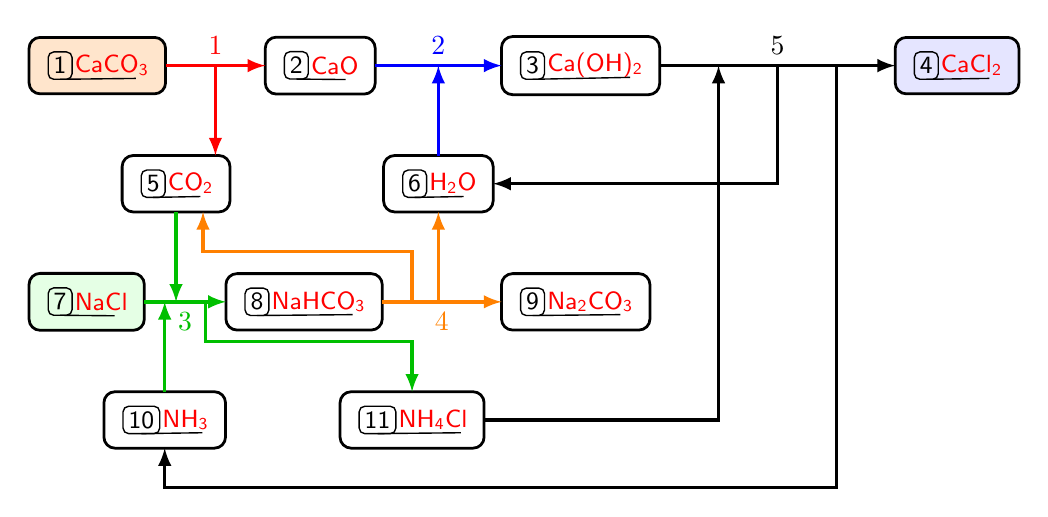
\begin{tikzpicture}[box/.style={draw=black, rectangle, rounded corners=4pt, line width=1pt, inner sep=5pt, outer sep=0pt},arrow/.style={-latex,very thick}]
 \node[box, right, fill=orange!20!white] (CaCO3) {\hl{\ce{CaCO3}}};
 \node[box, right] (CaO) at(3,0){\hl{\ce{CaO}}};
 \node[box, right] (CaOH2) at(6,0){\hl{\ce{Ca(OH)2}}};
 \node[box, right, fill=blue!10!white] (CaCl2) at(11,0){\hl{\ce{CaCl2}}};
 \draw[arrow, red] (CaCO3.east)--node[auto=left] {1}(CaO.west);
 \draw[arrow, blue] (CaO.east)--node[auto=left] {2}(CaOH2.west);
 \draw[arrow] (CaOH2.east)-- node[auto=left] {5}(CaCl2.west);
 
 \coordinate (1) at ($(CaCO3.east)!0.5!(CaO.west)$);
 \node[box] (CO2) at ([xshift=-5mm,yshift=-15mm]1){\hl{\ce{CO2}}};
 
 \coordinate (2) at ($(CaO.east)!0.5!(CaOH2.west)$);
 \node[box] (H2O) at ([yshift=-15mm]2){\hl{\ce{H2O}}};
 \draw[arrow, red] (1)--($(CO2.north)!(1)!(CO2.north east)$);
 \draw[arrow, blue] (H2O.north)--(2);
 \node[box, right, fill=green!10!white] (NaCl) at(0,-3) {\hl{\ce{NaCl}}};
 \node[box, right] (NaHCO3) at(2.5,-3){\hl{\ce{NaHCO3}}};
 \node[box, right] (Na2CO3) at(6,-3){\hl{\ce{Na2CO3}}};
 \draw[arrow, green!75!black] (NaCl.east)--node[auto=right] {3}(NaHCO3.west);
 \draw[arrow, orange] (NaHCO3.east)--node[auto=right] {4}(Na2CO3.west);
 
 \coordinate (3-1) at ($(NaCl.east)!0.25!(NaHCO3.west)$);
 \coordinate (3-3) at ($(NaCl.east)!0.75!(NaHCO3.west)$);
 \coordinate (4-2) at ($(NaHCO3.east)!0.25!(Na2CO3.west)$);
 \draw[arrow, green!75!black] (CO2.south)--($(NaCl.east)!(CO2.south)!(NaHCO3.west)$);
 \node[box] (NH3) at ([yshift=-15mm]3-1){\hl{\ce{NH3}}};
 \draw[arrow, green!75!black] (NH3.north)--(3-1.south);
 \node[box] (NH4Cl) at ([yshift=-15mm]4-2){\hl{\ce{NH4Cl}}};
 \draw[arrow, green!75!black] (3-3)--($(3-3)+(0,-0.5)$)-|(NH4Cl.north);
 \draw[arrow, orange] (4-2)|-($(CO2.south)!.5!(CO2.south east)+(0,-0.5)$)--($(CO2.south)!.5!(CO2.south east)$);
 \draw[arrow, orange] ($(NaHCO3.east)!(H2O.south)!(Na2CO3.west)$)--(H2O.south);
 \coordinate (5-1) at ($(CaOH2.east)!0.25!(CaCl2.west)$);
 \coordinate (5-2) at ($(CaOH2.east)!0.5!(CaCl2.west)$);
 \coordinate (5-3) at ($(CaOH2.east)!0.75!(CaCl2.west)$);
 \draw[arrow] (NH4Cl.east)-|(5-1);
 \draw[arrow] (5-2)|-(H2O.east);
 \draw[arrow] (5-3)|-($(NH3.south)+(0,-0.5)$)--(NH3.south);
\end{tikzpicture}
\begin{enumerate}
 \item \hl{炭酸カルシウム}の\hl{熱分解}\\
 \hce{CaCO3 -> CaO + CO2}
 \item \hl{酸化カルシウム}と\hl{水}\\
 \hce{CaO + H2O -> Ca(OH)2}
 \item \hl{塩化ナトリウム水溶液}に\hl{アンモニア}を溶解させてから、\hl{二酸化炭素}を溶解\\
 \hce{NaCl + NH3 + CO2 + H2O -> NH4Cl + NaHCO3 v}
 \item \hl{炭酸水素ナトリウム}の\hl{熱分解}\\
 \hce{2NaHCO3 -> Na2CO3 + H2O + CO2 ^}
 \item \hl{水酸化カルシウム}と\hl{塩化アンモニウム}\\
 \hce{2NH4Cl + Ca(OH)2 -> CaCl2 + 2NH3 ^ + 2H2O}
\end{enumerate}
\hce{2NaCl + CaCO3 -> CaCl2 + Na2CO3}
\end{itembox}

 \subsubsection{反応}
 \begin{itemize}
  \item \ce{Na2CO3}
  \begin{tabular}{ll}
  \hl{\ce{CO3^2- + H2O <=> HCO3- + OH-}}&$K_{1}=1.8\times10^{-4}$\\
  \end{tabular}
  \item \ce{NaHCO3}
  $\left\{
  \begin{tabular}{ll}
  \hl{\ce{HCO3- <=> H+ + CO3^{2-}}}&$K_{1}=5.6\times10^{-11}$\\
  \hl{\ce{HCO3- + H2O <=> CO2 + OH- + H2O}}&$K_{2}=2.3\times10^{-8}$
  \end{tabular}
  \right.$
 \end{itemize}
 
\newpage
 \section{2族元素}
 \hl{\ce{Be}},\hl{\ce{Mg}},\hl{アルカリ土類金属}
 \subsection{単体}
 \subsubsection{性質}
 \begin{tabular}{|c||c|c|c|c|c|}\hline
 化学式&\hl{\ce{Be}}&\hl{\ce{Mg}}&\hl{\ce{Ca}}&\hl{\ce{Sr}}&\hl{\ce{Ba}}\\ \hline
 融点&$1282^{\circ}$C&$649^{\circ}$C&$839^{\circ}$C&$769^{\circ}$C&$729^{\circ}$C\\ \hline
 密度(g/cm$^3$)&1.85&1.74&1.55&2.54&3.59\\ \hline
 \hl{還元}力&\multicolumn{5}{|c|}{小 \quad\tikz \draw[line width=0.5pt] (6,0.1)--(0,0)--(6,-0.1);\quad 大}\\ \hline
 水との反応&\hl{反応しない}&\hl{熱水}と反応&\hl{冷水}と反応&\hl{冷水}と反応&\hl{冷水}と反応\\ \hline
 \ce{M(OH)2}の水溶性&\multicolumn{2}{|c|}{\hl{難溶}性(\hl{弱塩基}性)}&\multicolumn{3}{|c|}{\hl{可溶}性(\hl{強塩基}性)}\\ \hline
 難溶性の塩&\multicolumn{2}{|c|}{\hl{\ce{MCO3}}}&\multicolumn{3}{|c|}{\hl{\ce{MCO3,MSO4}}}\\ \hline
 炎色反応&\hl{示さない}&\hl{示さない}&\hl{橙赤}&\hl{紅}&\hl{黄緑}\\ \hline
 用途&X線通過窓&フラッシュ&精錬の還元剤&発煙筒&ゲッター\\ \hline
 \end{tabular}
 \subsubsection{製法}
 塩化物の\hl{溶融塩電解} \K
 \subsubsection{反応}
 \begin{itemize}
  \item マグネシウムの燃焼\\
  \hce{2Mg + O2 -> 2 MgO}
  \item マグネシウムと二酸化炭素\\
  \hce{2Mg + CO2 -> 2 MgO + C}
  \item カルシウムと水\\
  \hce{Ca + 2H2O -> Ca(OH)2 + H2 ^}
 \end{itemize}
 
 \subsection{酸化カルシウム(生石灰)}
 化学式:\hl{\ce{CaO}}
 \subsubsection{性質}
 \begin{itemize}
  \item \hl{白}色
  \item \hl{水}との親和性が\hl{非常に高い}(\hl{乾燥剤})
  \item \hl{塩基性}酸化物
  \item 水との反応熱が\hl{非常に大きい}(\hl{加熱剤})
 \end{itemize}
 \subsubsection{製法}
 \hl{炭酸カルシウム}の\hl{熱分解}\\
 \hce{CaCO3 -> CaO + CO2}
 \subsubsection{反応}
 \begin{itemize}
  \item コークスを混ぜて強熱すると、\hl{炭化カルシウム}(\hl{カーバイド})が生成\\
  \hce{CaO + 3C -> CaC2 + CO ^}\\
  \hl{水}と反応して\hl{アセチレン}が生成\\
  \hce{CaC2 + 2H2O -> CaH2 ^ + Ca(OH2)2}
 \end{itemize}
 \subsection{水酸化カルシウム(消石灰)}
 化学式:\hl{\ce{Ca(OH)2}}
 \subsubsection{性質}
 \begin{itemize}
  \item \hl{白}色
  \item 水に\hl{少し溶ける}固体
  \item \hl{強塩基}
  $\left(
  \begin{tabular}{ll}
  \hl{\ce{Ca(OH)2 <=> Ca(OH)+ + OH-}}&$K_{1}=5.0\times10^{-2}$\\
  \end{tabular}
  \right)$
  \item 水溶液は\hl{石灰水}
 \end{itemize}
 \subsubsection{製法}
 \hl{酸化カルシウム}と\hl{水} \K\\
 \hce{CaO + H2O -> Ca(OH)2}
 \subsubsection{反応}
 \begin{itemize}
  \item 塩素と反応して、\hl{さらし粉}が生成\\
  \hce{Ca(OH)2 + Cl2 -> CaCl(ClO)*H2O}
  \item $580^{\circ}$C以上で\hl{熱分解}\\
  \hce{Ca(OH)2 -> CaO + H2O}
  \item 二酸化炭素との反応\\
  \hce{Ca(OH)2 + CO2 -> CaCO3 + H2O}
  \item 塩化アンモニウムとの反応\\
  \hce{2NH4Cl + Ca(OH)2 -> CaCl2 + 2NH3 ^ + 2H2O}
 \end{itemize}
 \subsection{炭酸カルシウム(石灰石)}
 化学式:\hl{\ce{CaCO3}}
 \subsubsection{性質}
 \begin{itemize}
  \item \hl{白}色で、水に\hl{溶けにくい}
  \item \hl{鍾乳洞}の形成
 \end{itemize}
 \subsubsection{反応}
 \begin{itemize}
  \item $800^{\circ}$C以上で\hl{熱分解}\\
  \hce{CaCO3 -> CaO + CO2}
  \item \hl{二酸化炭素}を多く含む水に\hl{溶解}\\
  \hce{CaCO3 + CO2 + H2O <=> Ca(HCO3)2}
 \end{itemize}
 \subsection{塩化マグネシウム・塩化カルシウム}
 化学式:\hl{\ce{MgCl2}}・\hl{\ce{CaCl2}}
 \subsubsection{性質}
  \hl{潮解}性があり、水に\hl{よく溶ける}(水との親和性が\hl{非常に高い})\\
  \hl{乾燥}剤 \stamp{teal}{塩化カルシウム}、\hl{融雪}剤
 \subsubsection{製法}
 \begin{itemize}
  \item 海水から得た\hl{にがり}を濃縮 \stamp{teal}{塩化マグネシウム} \K
  \item \hl{アンモニアソーダ法}(\hl{ソルベー法})\stamp{teal}{塩化カルシウム} \K
 \end{itemize}
 \subsection{硫酸カルシウム}
 化学式:\hl{\ce{CaSO4}}
 \subsubsection{性質}
  \hl{セッコウ}を約$150^{\circ}$Cで加熱すると、\hl{焼きセッコウ}が生成\\
  \hl{水}を加えると、\hl{発熱}・\hl{膨張}・\hl{硬化}して\hl{セッコウ}に戻る\\
  \hce{CaSO4*2H2O <=>T[$\Delta$][硬化] CaSO4*$\dfrac{1}{2}$H2O + $\dfrac{3}{2}$H2O}\\
  \stamp{red}{用途} 医療用ギプス・石膏像・建材
 \subsection{硫酸バリウム}
 化学式:\hl{\ce{BaSO4}}
 \subsubsection{性質}
 \begin{itemize}
  \item \hl{白}色で、水に\hl{ほとんど溶けない}固体
  \item 反応性が\hl{低}く、X線を遮蔽
 \end{itemize}
 \section{12族元素}
 \subsection{単体}
 \subsubsection{性質}
 \begin{tabular}{|c|c|c|c|}\hline
 化学式&\hl{\ce{Zn}}&\hl{\ce{Cd}}&\hl{\ce{Hg}}\\ \hline
 融点&$420^\circ$C&$321^\circ$C&$-39^\circ$C\\ \hline
 密度&7.1&8.6&13.6\\ \hline
 \ce{M^{2+}aq + H2S}&\hl{白}色の\hl{\ce{ZnS}}\ce{v}&\hl{黄}色の\hl{\ce{CdS}}\ce{v}&\hl{黒}色の\hl{\ce{HgS}}\ce{v}\\
 (沈澱条件)&(\hl{中塩基性})&(\hl{全液性})&(\hl{全液性})\\ \hline
 \multirow{2}{*}{特性}&高温の水蒸気と反応&\ce{Cd^2+}は\ce{Ca^2+}と類似&\hl{合金}を作りやすい\\
 &\hl{両性}元素&$\Rightarrow$イタイイタイ病&(\hl{アマルガム})\\ \hline
 用途&\hl{トタン}(鉄にメッキ)&ニカド電池 (Ni-Cd)&体温計・蛍光灯\\ \hline
 \end{tabular}
 \begin{itemize}
  \item 12族の硫化物は\hl{顔料}や\hl{染料}に利用
  \item \ce{HgS}は$450^\circ$Cで消火させると\hl{赤}色に変化
 \end{itemize}
 \subsubsection{製法}
 閃亜鉛鉱を焙焼して得た酸化亜鉛に、コークスを混ぜて加工 \K
 \hce{2ZnS + 3O2 -> 2ZnO + 2SO2}\\
 \hce{ZnO + C -> Zn + CO}
 \subsubsection{反応}
 \begin{itemize}
  \item 高温の水蒸気と反応\\
  \hce{Zn + H2O -> ZnO + H2 ^}
  \item 塩酸と反応\\
  \hce{Zn + 2HCl -> ZnCl2 + H2 ^}
  \item 水酸化ナトリウム水溶液と反応\\
  \hce{Zn + 2NaOH + 2H2O -> Na2[Zn(OH)4] + H2 ^}
 \end{itemize}
 \subsection{酸化亜鉛(亜鉛華)・水酸化亜鉛}
 化学式:\hl{\ce{ZnO}}・\hl{\ce{Zn(OH)2}}
 \subsubsection{性質}
 \begin{itemize}
  \item \hl{白}色で、水に\hl{とけにくい}固体
  \item 酸化亜鉛は\hl{顔料}
  \item \hl{両性}酸化物・\hl{両性}水酸化物\\
  \hl{酸}・(強)\hl{塩基}と反応
  \ce{Zn^2+}は、\hl{\ce{OH-}}とも\hl{\ce{NH3}}とも錯イオンを形成
 \end{itemize}
 \subsubsection{製法}
 \begin{itemize}
  \item 亜鉛を燃焼 \K  \stamp{teal}{酸化亜鉛}\\
  \hce{2Zn + O2 -> 2ZnO}
  \item 亜鉛イオンを含む水溶液に、少量の\hl{\ce{OH-}}を加える \stamp{teal}{水酸化亜鉛}\\
  \hce{Zn^2+ + 2OH- -> Zn(OH)2 v}
 \end{itemize}
 \subsubsection{反応}
 \begin{itemize}
  \item 酸化亜鉛と塩酸\\
  \hce{ZnO + 2HCl -> ZnCl2 + H2O}
  \item 酸化亜鉛と水酸化ナトリウム水溶液\\
  \hce{ZnO + 2NaOH + H2O -> Na2[Zn(OH)4]}
  \item 水酸化亜鉛と塩酸\\
  \hce{Zn(OH)2 + 2HCl -> ZnCl2 + 2H2O}
  \item 水酸化亜鉛と水酸化ナトリウム水溶液\\
  \hce{Zn(OH)2 + 2NaOH -> Na2[Zn(OH)4]}
  \item 水酸化亜鉛の過剰な\hl{アンモニア}との反応\\
  \hce{Zn(OH)2 + 4NH3 -> [Zn(NH3)4](OH)2}
 \end{itemize}
 \subsection{塩化水銀(\UTF{2160})・塩化水銀(\UTF{2161})}
 化学式:\hl{\ce{Hg2Cl2}}・\hl{\ce{HgCl}}
 \subsubsection{性質}
 \begin{itemize}
  \item 白色で、水に溶けにくい固体で、微毒
  \item 白色で、水に少し溶ける固体で、猛毒
 \end{itemize}
 \subsubsection{製法}
 水酸化銀(\ajRoman{2})と水銀の混合物を加熱\\
 \hce{HgCl2 + Hg -> Hg2Cl2}
 \section{アルミニウム}
 \subsection{アルミニウム}
 \subsection{酸化アルミニウム}
 \subsection{ミョウバン}
 \section{スズ・鉛}
 \onecolumn
 \setcounter{section}{0}
 \part{APPENDIX}
  \section{気体の乾燥剤}
  固体の乾燥剤は\hl{U字管}につめて、液体の乾燥剤は\hl{洗気瓶}に入れて使用。\\
  \begin{tabular}{|c|cc|c|c|}\hline
  性質&乾燥剤&化学式&対象&対象外(不適)\\ \hline
  \multirow{2}{*}{酸性}&\hl{十酸化四リン}&\hl{\ce{P4O10}}&\multirow{2}{*}{酸性・中性}&塩基性の気体(\hl{\ce{NH3}})\\ \cline{2-3} \cline{5-5}
  &\hl{濃硫酸}&\hl{\ce{H2SO4}}&&+\hl{\ce{H2S}}(\hl{還元剤})\\ \hline
  \multirow{2}{*}{中性}&\hl{塩化カルシウム}&\hl{\ce{CaCl2}}&\multirow{2}{*}{ほとんど全て}&\hl{\ce{NH3}}\\ \cline{2-3} \cline{5-5}
  &\hl{シリカゲル}&\hl{\ce{SiO2*$n$H2O}}&&特になし\\ \hline
  \multirow{2}{*}{塩基性}&\hl{酸化カルシウム}&\hl{\ce{CaO}}&\multirow{2}{*}{中性・塩基性}&酸性の気体\\ \cline{2-3}
  &\hl{ソーダ石灰}&\hl{\ce{CaO}と\ce{NaOH}}&&\hl{\ce{Cl2}},\hl{\ce{HCl}},\hl{\ce{H2S}},\hl{\ce{SO2}},\hl{\ce{CO2}},\hl{\ce{NO2}}\\ \hline
  \end{tabular}
  \section{水の硬度}
  水の中の重荷\ce{Ca^2+}と\ce{Mg^2+}を\ce{CaCO3}として換算した時の濃度[mg/L]\\
  硬水に含まれる陰イオンが
  $\left\{
  \begin{tabular}{l}
  煮沸する\hl{炭酸塩}が沈澱して軟化可能(一時硬水)\\
  $\left(
  \begin{tabular}{l}
   \R 炭酸水素カルシウム水溶液\\
   \hce{Ca(HCO3)2 -> CaCO3 v + H2O + CO2}\\
   \R 炭酸水素マグネシウム水溶液\\
   \hce{Mg(HCO3)2 -> MgCO3 v + H2O + CO2}
  \end{tabular}
  \right)$\\
  煮沸しても軟化不可能(永久硬水)
  \end{tabular}
  \right.$
  \section{錯イオンの命名法}
  (主に遷移)金属イオンに対して、\hl{非共有電子対}を持つ\hl{分子}や\hl{イオン}が\hl{配位}結合\\
  「 \stamp{OrangeRed}{配位子の数(数詞)} \stamp{YellowOrange}{配位子} \stamp{YellowGreen}{金属(価数)} \stamp{Cerulean}{酸(陰イオンの場合)}イオン」\\\\
  \begin{tabular}{|c|cc|cc|cccccc|}\hline
  金属イオン&\ce{Ag+}&\ce{Cu+}&\ce{Cu^2+}&\ce{Zn^2+}&\ce{Fe^2+}&\ce{Fe^3+}&\ce{Co^3+}&\ce{Ni^2+}&\ce{Cr^3+}&\ce{Al^3+}\\ \hline
  配位数&\multicolumn{2}{|c|}{\hl{2}}&\multicolumn{2}{|c|}{\hl{4}}&\multicolumn{6}{|c|}{\hl{6}}\\ \hline
  \multicolumn{1}{c}{}&\multicolumn{2}{c}{\hl{直線}系}&\hl{正方}形&\multicolumn{1}{c}{\hl{正四面体}形}&\multicolumn{6}{c}{\hl{正八面体}形}
  \end{tabular}\\
  \begin{tabular}{|c|c|c|c|c|c|c|c|c|}\hline
  数&1&2&3&4&5&6&7&8\\ \hline
  数詞&\hl{モノ}&\hl{ジ}&\hl{トリ}&\hl{テトラ}&\hl{ペンタ}&\hl{ヘキサ}&\hl{ヘプタ}&\hl{オクタ}\\
  &&\hl{ビス}&\hl{トリス}&&&&&\\ \hline
  \end{tabular}\\
  \begin{tabular}{|c|c|c|c|c|c|c|}\hline
  配位子&\ce{NH3}&\ce{CN-}&\ce{H2O}&\ce{OH-}&\ce{Cl-}&\ce{H2N - CH2CH2 - NH2}\\ \hline
  名称&\hl{アンミン}&\hl{シアニド}&\hl{アクア}&\hl{ヒドロキシド}&\hl{クロリド}&\hl{エチレンジアミン}\\ \hline
  \end{tabular}\\
  エチレンジアミン$\cdots$1分子あたり2か所で\hl{配位}結合する(2座配位子)\\(\hl{キレート}錯体)
  \hlbox{\chemfig{
  Cu(-[1,1.5,,,<-]{NH_{2}}-[:120]{CH_{2}}?[a])(-[3,1.5,,,<-]{H_{2}N}-[:60]{H_{2}C}?[a])(-[-1,1.5,,,<-]{NH_{2}}-[:-120]{CH_{2}}?[b])(-[-3,1.5,,,<-]{H_{2}N}-[:-60]{H_{2}C}?[b])
  }}
  \begin{itemize}
   \item \ce{[Zn(OH)4]^2-}\\
   \hl{テトラヒドロキシド亜鉛(\ajRoman{2})酸イオン}
   \item \ce{[Zn(NH3)4]^2+}\\
   \hl{テトラアンミン亜鉛(\ajRoman{2})イオン}
   \item \ce{[Ag(S2O3)2]^3-}\\
   \hl{ビス(チオスルファト)銀(\ajRoman{1})イオン}
   \item \ce{[Cu(H2NCH2CH2NH2)]^2+}\\
   \hl{ビス(エチレンジアミン)銅(\ajRoman{2})イオン}
  \end{itemize}
\end{document}